

Line $k$ is defined by $y=-\frac{17}{3} x+5$. Line $j$ is perpendicular to line $k$ in the $x y$-plane. What is the slope of line $j$ ?

\section*{ID: 3008cfc3}
\begin{center}
\begin{tabular}{|c|c|}
\hline
$x$ & $y$ \\
\hline
$k$ & 13 \\
\hline
$k+7$ & -15 \\
\hline
\end{tabular}
\end{center}

The table gives the coordinates of two points on a line in the $x y$-plane. The $y$-intercept of the line is $(k-5, b)$, where $k$ and $b$ are constants. What is the value of $b$ ?

\section*{ID: 3cdbf026}
The graph of the equation $a x+k y=6$ is a line in the $x y$-plane, where $a$ and $k$ are constants. If the line contains the points $(-2,-6)$ and $(0,-3)$, what is the value of $k$ ?\\
A. -2\\
B. -1\\
C. 2\\
D. 3

\section*{ID: 9bbce683}
\begin{center}
\begin{tabular}{|c|c|}
\hline
$x$ & $y$ \\
\hline
18 & 130 \\
\hline
23 & 160 \\
\hline
26 & 178 \\
\hline
\end{tabular}
\end{center}

For line $h$, the table shows three values of $x$ and their corresponding values of $y$. Line $k$ is the result of translating line $h$ down 5 units in the $x y$-plane. What is the $x$-intercept of line $k$ ?\\
A. $\left(-\frac{26}{3}, 0\right)$\\
B. $\left(-\frac{9}{2}, 0\right)$\\
C. $\left(-\frac{11}{3}, 0\right)$\\
D. $\left(-\frac{17}{6}, 0\right)$

\section*{ID: 686b7244}
A certain apprentice has enrolled in 85 hours of training courses. The equation $10 x+15 y=85$ represents this situation, where $x$ is the number of on-site training courses and $y$ is the number of online training courses this apprentice has enrolled in. How many more hours does each online training course take than each on-site training course?

\section*{ID: ee846db7}
A store sells two different-sized containers of a certain Greek yogurt. The store's sales of this Greek yogurt totaled $1,277.94$ dollars last month. The equation $5.48 x+7.30 y=1,277.94$ represents this situation, where $x$ is the number of smaller containers sold and $y$ is the number of larger containers sold. According to the equation, which of the following represents the price, in dollars, of each smaller container?\\
A. 5.48\\
B. $7.30 y$\\
C. 7.30\\
D. $5.48 x$

Line $k$ is defined by $y=3 x+15$. Line $j$ is perpendicular to line $k$ in the $x y$-plane. What is the slope of line $j$ ?\\
A. $-\frac{1}{3}$\\
B. $-\frac{1}{12}$\\
C. $-\frac{1}{18}$\\
D. $-\frac{1}{45}$

Line $p$ is defined by $4 y+8 x=6$. Line $r$ is perpendicular to line $p$ in the $x y$-plane. What is the slope of line $r$ ?

Line $p$ is defined by $2 y+18 x=9$. Line $r$ is perpendicular to line $p$ in the $x y$-plane. What is the slope of line $r$ ?\\
A. -9\\
B. $-\frac{1}{9}$\\
C. $\frac{1}{9}$\\
D. 9

$$
y=x+4
$$

Which table gives three values of $x$ and their corresponding values of $y$ for the given equation?\\
A.

\begin{center}
\begin{tabular}{|c|c|}
\hline
$x$ & $y$ \\
\hline
0 & 4 \\
\hline
1 & 5 \\
\hline
2 & 6 \\
\hline
\end{tabular}
\end{center}

B.

\begin{center}
\begin{tabular}{|c|c|}
\hline
$x$ & $y$ \\
\hline
0 & 6 \\
\hline
1 & 5 \\
\hline
2 & 4 \\
\hline
\end{tabular}
\end{center}

c.

\begin{center}
\begin{tabular}{|c|c|}
\hline
$x$ & $y$ \\
\hline
0 & 2 \\
\hline
1 & 1 \\
\hline
2 & 0 \\
\hline
\end{tabular}
\end{center}

D.

\begin{center}
\begin{tabular}{|c|c|}
\hline
$x$ & $y$ \\
\hline
0 & 0 \\
\hline
1 & 1 \\
\hline
2 & 2 \\
\hline
\end{tabular}
\end{center}

































\section*{ID: 9c7741c6}
On a 210-mile trip, Cameron drove at an average speed of 60 miles per hour for the first $x$ hours. He then completed the trip, driving at an average speed of 50 miles per hour for the remaining $y$ hours. If $x=1$, what is the value of $y$ ?

The $y$-intercept of the graph of $12 x+2 y=18$ in the $x y$-plane is $(0, y)$. What is the value of $y$ ?

In the $x y$-plane, line $\ell$ passes through the point $(0,0)$ and is parallel to the line represented by the equation $y=8 x+2$. If line $\ell$ also passes through the point $(3, d)$, what is the value of $d$ ?\\
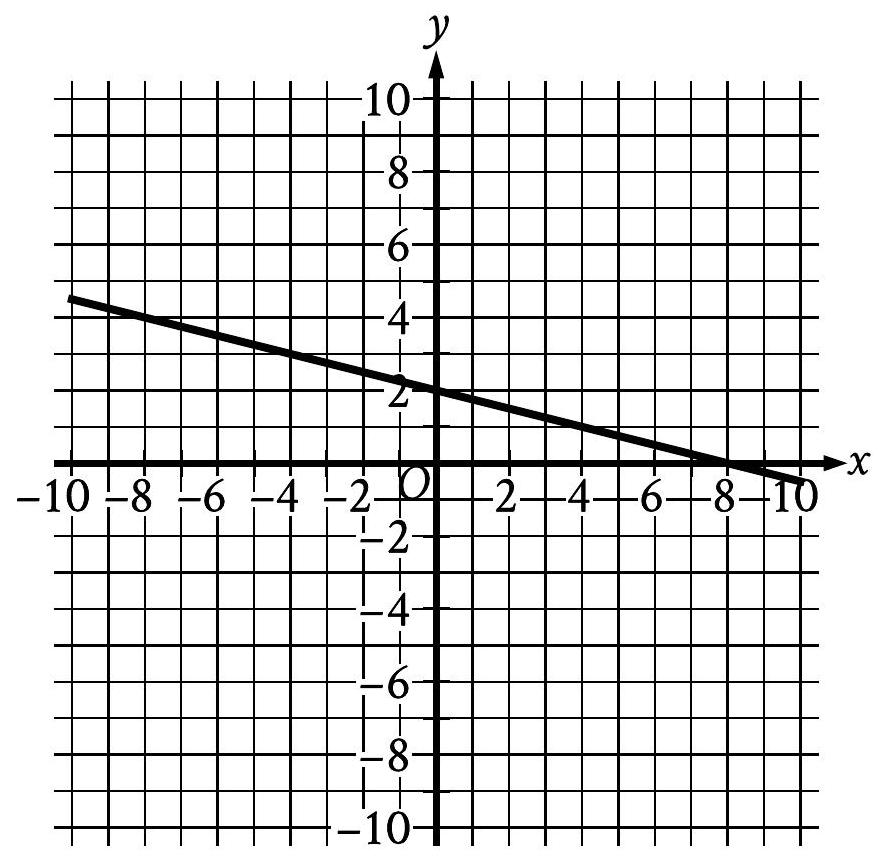
\includegraphics[max width=\textwidth, center]{2025_06_15_8c4b9d94a674ec08620fg-24}

The graph of $y=f(x)+14$ is shown. Which equation defines function $f$ ?\\
A. $f(x)=-\frac{1}{4} x-12$\\
B. $f(x)=-\frac{1}{4} x+16$\\
C. $f(x)=-\frac{1}{4} x+2$\\
D. $f(x)=-\frac{1}{4} x-14$

\section*{ID: cc7ffe02}
Keenan made 32 cups of vegetable broth. Keenan then filled $x$ small jars and $y$ large jars with all the vegetable broth he made. The equation $3 x+5 y=32$ represents this situation. Which is the best interpretation of $5 y$ in this context?\\
A. The number of large jars Keenan filled\\
B. The number of small jars Keenan filled\\
C. The total number of cups of vegetable broth in the large jars\\
D. The total number of cups of vegetable broth in the small jars\\
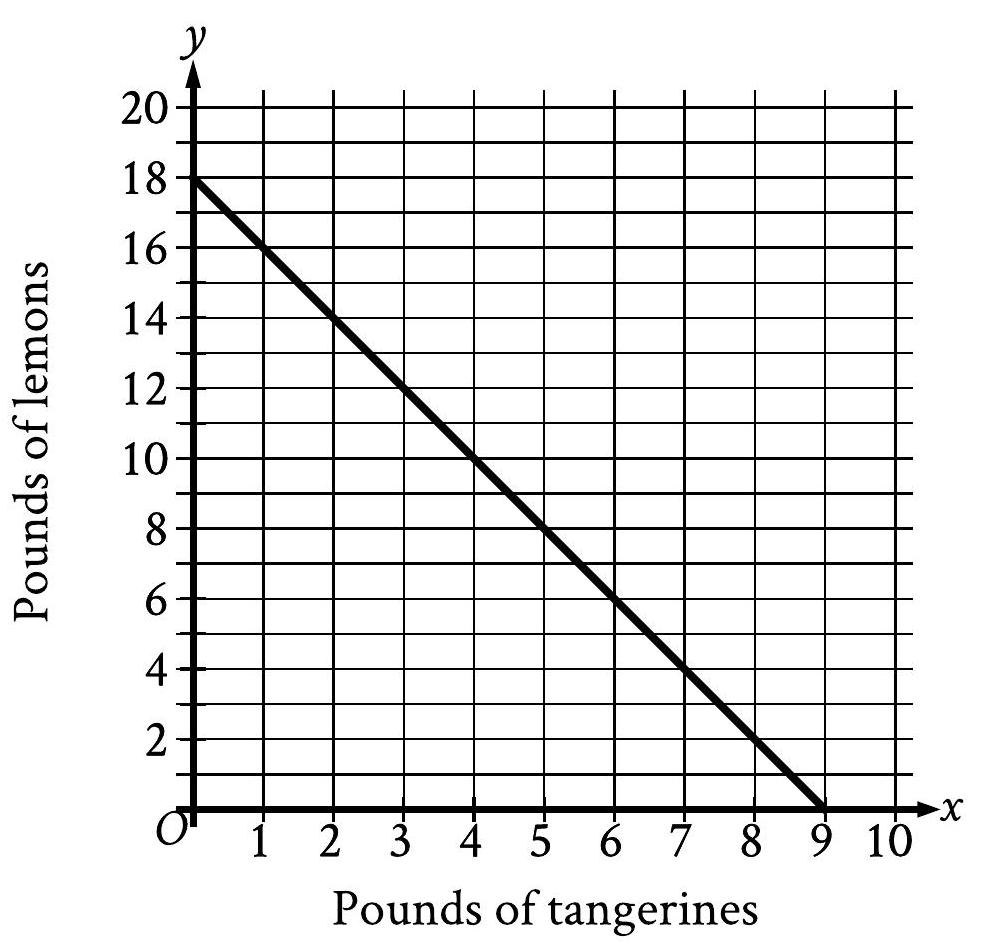
\includegraphics[max width=\textwidth, center]{2025_06_15_8c4b9d94a674ec08620fg-26}

The graph shows the possible combinations of the number of pounds of tangerines and lemons that could be purchased for $\$ 18$ at a certain store. If Melvin purchased lemons and 4 pounds of tangerines for a total of $\$ 18$, how many pounds of lemons did he purchase?\\
A. 7\\
B. 10\\
C. 14\\
D. 16\\
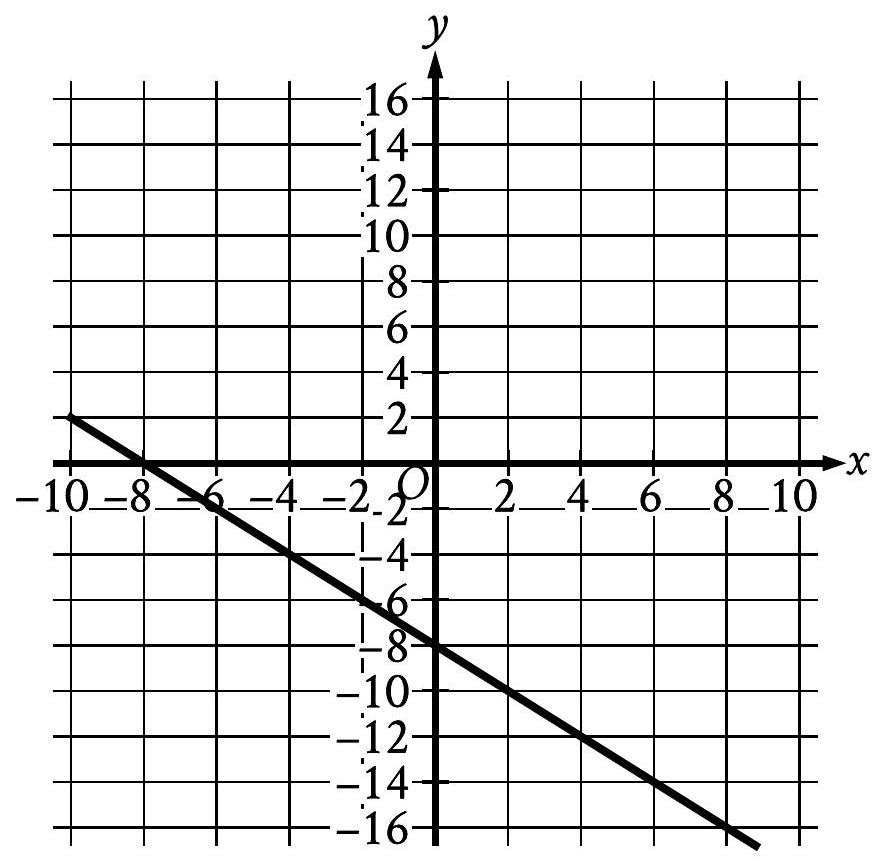
\includegraphics[max width=\textwidth, center]{2025_06_15_8c4b9d94a674ec08620fg-27}

What is an equation of the graph shown?\\
A. $y=-2 x-8$\\
B. $y=x-8$\\
C. $y=-x-8$\\
D. $y=2 x-8$

\section*{ID: 8adf1335}
A city's total expense budget for one year was $x$ million dollars. The city budgeted $y$ million dollars for departmental expenses and 201 million dollars for all other expenses. Which of the following represents the relationship between $x$ and $y$ in this context?\\
A. $x+y=201$\\
B. $x-y=201$\\
C. $2 x-y=201$\\
D. $y-x=201$

ID: 0b46bad5\\
$a x+b y=b$

In the equation above, $a$ and $b$ are constants and $0<a<b$. Which of the following could represent the graph of the equation in the $x y$-plane?\\
A.\\
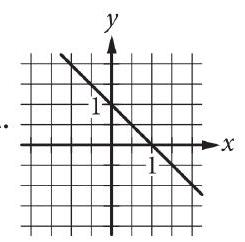
\includegraphics[max width=\textwidth, center]{2025_06_15_8c4b9d94a674ec08620fg-29(3)}\\
B.\\
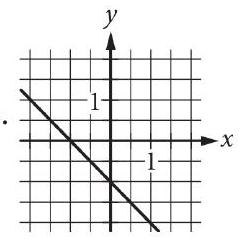
\includegraphics[max width=\textwidth, center]{2025_06_15_8c4b9d94a674ec08620fg-29}\\
C.\\
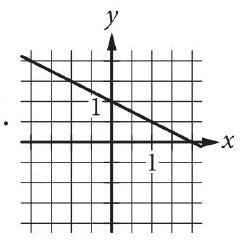
\includegraphics[max width=\textwidth, center]{2025_06_15_8c4b9d94a674ec08620fg-29(1)}\\
D.\\
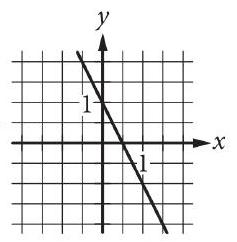
\includegraphics[max width=\textwidth, center]{2025_06_15_8c4b9d94a674ec08620fg-29(2)}

$$
y=-4 x+40
$$

Which table gives three values of $x$ and their corresponding values of $y$ for the given equation?\\
A.

\begin{center}
\begin{tabular}{|c|c|}
\hline
$x$ & $y$ \\
\hline
0 & 0 \\
\hline
1 & -4 \\
\hline
2 & -8 \\
\hline
\end{tabular}
\end{center}

B.

\begin{center}
\begin{tabular}{|c|c|}
\hline
$x$ & $y$ \\
\hline
0 & 40 \\
\hline
1 & 44 \\
\hline
2 & 48 \\
\hline
\end{tabular}
\end{center}

c.

\begin{center}
\begin{tabular}{|c|c|}
\hline
$x$ & $y$ \\
\hline
0 & 40 \\
\hline
1 & 36 \\
\hline
2 & 32 \\
\hline
\end{tabular}
\end{center}

D.

\begin{center}
\begin{tabular}{|c|c|}
\hline
$x$ & $y$ \\
\hline
0 & 0 \\
\hline
1 & 4 \\
\hline
2 & 8 \\
\hline
\end{tabular}
\end{center}

Number of Cornflowers and Wallflowers at Garden Store\\
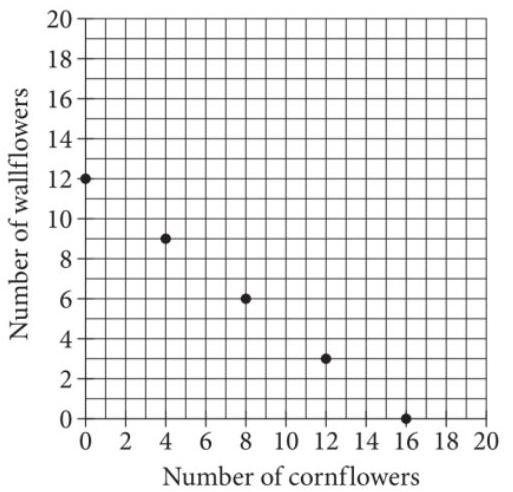
\includegraphics[max width=\textwidth, center]{2025_06_15_8c4b9d94a674ec08620fg-31}

The points plotted in the coordinate plane above represent the possible numbers of wallflowers and cornflowers that someone can buy at the Garden Store in order to spend exactly $\$ 24.00$ total on the two types of flowers. The price of each wallflower is the same and the price of each cornflower is the same. What is the price, in dollars, of 1 cornflower?

The graph of $7 x+2 y=-31$ in the $x y$-plane has an $x$-intercept at $(a, 0)$ and a $y$-intercept at $(0, b)$, where $a$ and $b$ are constants. What is the value of $\frac{b}{a}$ ?\\
A. $-\frac{7}{2}$\\
B. $-\frac{2}{7}$\\
C. $\frac{2}{7}$\\
D. $\frac{7}{2}$\\
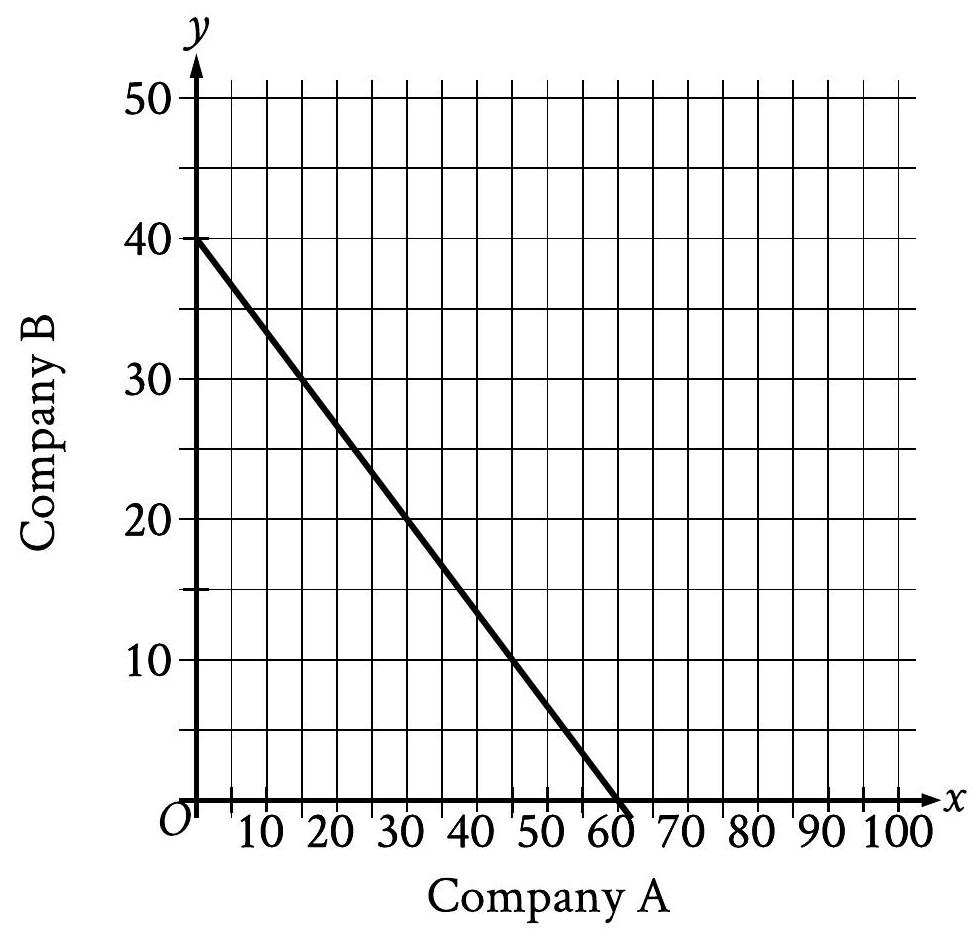
\includegraphics[max width=\textwidth, center]{2025_06_15_8c4b9d94a674ec08620fg-33}

The graph shows the relationship between the number of shares of stock from Company A , $x$, and the number of shares of stock from Company B, $y$, that Simone can purchase. Which equation could represent this relationship?\\
A. $y=8 x+12$\\
B. $8 x+12 y=480$\\
C. $y=12 x+8$\\
D. $12 x+8 y=480$

\section*{ID: dd797fe2}
$4 x+3 y=24$

Mario purchased 4 binders that cost $x$ dollars each and 3 notebooks that cost $y$ dollars each. If the given equation represents this situation, which of the following is the best interpretation of 24 in this context?\\
A. The total cost, in dollars, for all binders purchased\\
B. The total cost, in dollars, for all notebooks purchased\\
C. The total cost, in dollars, for all binders and notebooks purchased\\
D. The difference in the total cost, in dollars, between the number of binders and notebooks purchased

\section*{ID: 789975b7}
A gardener buys two kinds of fertilizer. Fertilizer A contains $60 \%$ filler materials by weight and Fertilizer B contains $40 \%$ filler materials by weight. Together, the fertilizers bought by the gardener contain a total of 240 pounds of filler materials. Which equation models this relationship, where $x$ is the number of pounds of Fertilizer A and $y$ is the number of pounds of Fertilizer B?\\
A. $0.4 x+0.6 y=240$\\
B. $0.6 x+0.4 y=240$\\
C. $40 x+60 y=240$\\
D. $60 x+40 y=240$

In the $x y$-plane, a line has a slope of 6 and passes through the point $(0,8)$. Which of the following is an equation of this line?\\
A. $y=6 x+8$\\
B. $y=6 x+48$\\
C. $y=8 x+6$\\
D. $y=8 x+48$

\section*{ID: d62ad380}
An artist paints and sells square tiles. The selling price $P$, in dollars, of a painted tile is a linear function of the side length of the tile $s$, in inches, as shown in the table below.

\begin{center}
\begin{tabular}{|c|c|}
\hline
Side length, $s$ (inches) & Price, $P$ (dollars) \\
\hline
3 & 8.00 \\
\hline
6 & 18.00 \\
\hline
9 & 28.00 \\
\hline
\end{tabular}
\end{center}

Which of the following could define the relationship between $s$ and $P$ ?\\
A. $P=3 s+10$\\
B. $P=\frac{10}{3} s+8$\\
c. $P=\frac{10}{3} s-2$\\
D. $P=\frac{3}{10} s-\frac{1}{10}$

The equation $40 x+20 y=160$ represents the number of sweaters, $x$, and number of shirts, $y$, that Yesenia purchased for $\$ 160$. If Yesenia purchased 2 sweaters, how many shirts did she purchase?\\
A. 3\\
B. 4\\
C. 8\\
D. 40

\section*{ID: ba79f10f}
\begin{center}
\begin{tabular}{|c|c|}
\hline
$x$ & $y$ \\
\hline
0 & 18 \\
\hline
1 & 13 \\
\hline
2 & 8 \\
\hline
\end{tabular}
\end{center}

The table shows three values of $x$ and their corresponding values of $y$. There is a linear relationship between $x$ and $y$. Which of the following equations represents this relationship?\\
A. $y=18 x+13$\\
B. $y=18 x+18$\\
C. $y=-5 x+13$\\
D. $y=-5 x+18$

Line $\ell$ in the $x y$-plane is perpendicular to the line with equation $x=2$. What is the slope of line $\ell$ ?\\
A. 0\\
B. $-\frac{1}{2}$\\
C. -2\\
D. The slope of line $\ell$ is undefined.

\section*{ID: dfa45424}
Tony spends $\$ 80$ per month on public transportation. A 10 -ride pass costs $\$ 12.50$, and a single-ride pass costs $\$ 1.50$. If $g$ represents the number of 10 -ride passes Tony buys in a month and $t$ represents the number of single-ride passes Tony buys in a month, which of the following equations best represents the relationship between $g$ and $t$ ?\\
A. $g+t=80$\\
B. $g+t=1.50+12.50$\\
C. $1.50 \mathrm{~g}+12.50 \mathrm{t}=80$\\
D. $12.50 g+1.50 t=80$

In an article about exercise, it is estimated that a 160-pound adult uses 200 calories for every 30 minutes of hiking and 150 calories for every 30 minutes of bicycling. An adult who weighs 160 pounds has completed 1 hour of bicycling. Based on the article, how many hours should the adult hike to use a total of 1,900 calories from bicycling and hiking?\\
A. 9.5\\
B. 8.75\\
C. 6\\
D. 4

The graph of $9 x-10 y=19$ is translated down 4 units in the $x y$-plane. What is the $x$-coordinate of the $x$-intercept of the resulting graph?

Characteristics for Rock Types

\begin{center}
\begin{tabular}{|c|c|c|}
\hline
Rock type & \begin{tabular}{c}
Weight per volume \\
(lb/ft $^{\mathbf{3}}$ ) \\
\end{tabular} & \begin{tabular}{c}
Cost per \\
pound \\
\end{tabular} \\
\hline
Basalt & 180 & $\$ 0.18$ \\
\hline
Granite & 165 & $\$ 0.09$ \\
\hline
Limestone & 120 & $\$ 0.03$ \\
\hline
Sandstone & 135 & $\$ 0.22$ \\
\hline
\end{tabular}
\end{center}

A city is planning to build a rock retaining wall, a monument, and a garden in a park. The table above shows four rock types that will be considered for use in the project. Also shown for each rock type is its weight per volume, in pounds per cubic foot $\left(\mathrm{lb} / \mathrm{ft}^{3}\right)$, and the cost per pound, in dollars. The equation $0.03(120 w)+0.18(180 z)+3,385.80=7,576.20$ gives the total cost, in dollars, of the rocks used in the project in terms of the number of $\mathrm{ft}^{3}$ of limestone, $w$, and the number of $\mathrm{ft}^{3}$ of basalt, z. All four rock types are used in the project. Which of the following is the best interpretation of $3,385.80$ in this context?\\
A. The cost of the granite and sandstone needed for the project\\
B. The cost of the basalt and limestone needed for the project\\
C. The cost of the basalt needed for the project\\
D. The cost of the sandstone needed for the project

When line $n$ is graphed in the $x y$-plane, it has an $x$-intercept of $(-4,0)$ and a $y$-intercept of $\left(0, \frac{86}{3}\right)$. What is the slope of line $n$ ?\\
A. $\frac{3}{344}$\\
B. $\frac{6}{43}$\\
C. $\frac{43}{6}$\\
D. $\frac{344}{3}$

\section*{ID: f81a0503}
In the $x y$-plane, line $k$ passes through the points $(0,-5)$ and $(1,-1)$. Which equation defines line $k$ ?\\
A. $y=-x+\frac{1}{4}$\\
B. $y=\frac{1}{4} x-5$\\
C. $y=-x+4$\\
D. $y=4 x-5$

\begin{center}
\begin{tabular}{|c|c|}
\hline
$x$ & $y$ \\
\hline
3 & 7 \\
\hline
$k$ & 11 \\
\hline
12 & $n$ \\
\hline
\end{tabular}
\end{center}

The table above shows the coordinates of three points on a line in the $x y$-plane, where $k$ and $n$ are constants. If the slope of the line is 2 , what is the value of $k+n$ ?

\section*{ID: 10c448d6}
A line in the $x y$-plane has a slope of $\frac{1}{9}$ and passes through the point $(0,14)$. Which equation represents this line?\\
A. $y=-\frac{1}{9} x-14$\\
B. $y=-\frac{1}{9} x+14$\\
C. $y=\frac{1}{9} x-14$\\
D. $y=\frac{1}{9} x+14$

Vivian bought party hats and cupcakes for $\$ 71$. Each package of party hats cost $\$ 3$, and each cupcake cost $\$ 1$. If Vivian bought 10 packages of party hats, how many cupcakes did she buy?\\
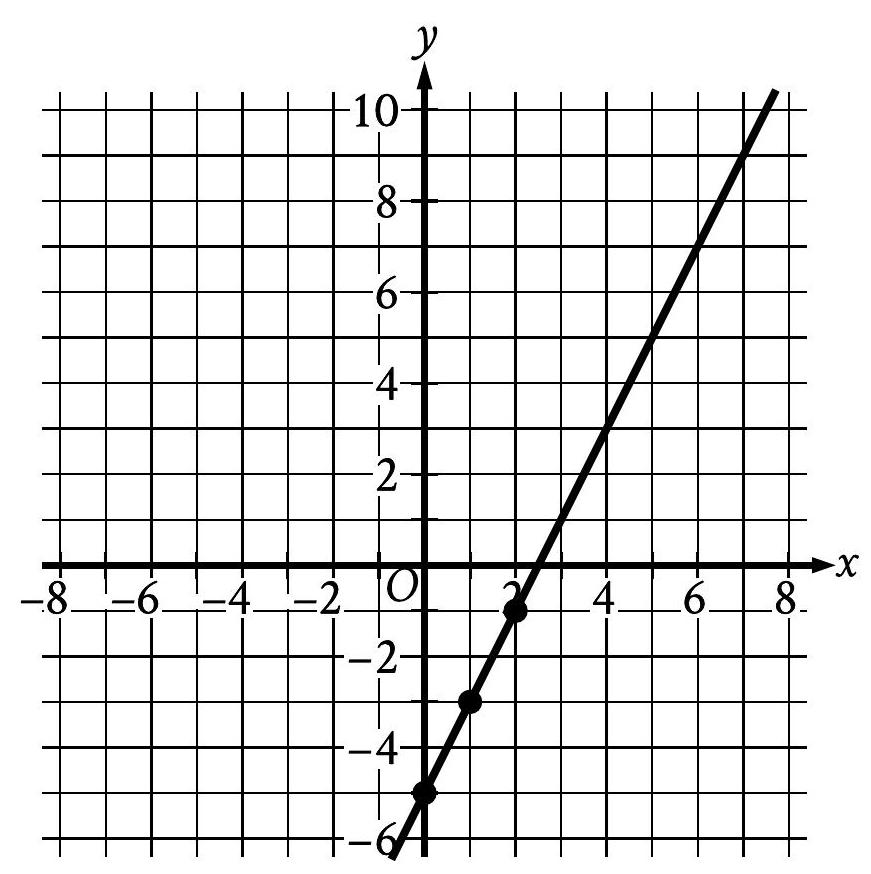
\includegraphics[max width=\textwidth, center]{2025_06_15_8c4b9d94a674ec08620fg-50}

The graph shows the linear relationship between $x$ and $y$. Which table gives three values of $x$ and their corresponding values of $y$ for this relationship?\\
A.

\begin{center}
\begin{tabular}{|c|c|}
\hline
$x$ & $y$ \\
\hline
0 & 0 \\
\hline
1 & -7 \\
\hline
2 & -9 \\
\hline
\end{tabular}
\end{center}

B.

\begin{center}
\begin{tabular}{|c|c|}
\hline
$x$ & $y$ \\
\hline
0 & 0 \\
\hline
1 & -3 \\
\hline
2 & -1 \\
\hline
\end{tabular}
\end{center}

C.

\begin{center}
\begin{tabular}{|c|c|}
\hline
$x$ & $y$ \\
\hline
0 & -5 \\
\hline
1 & -7 \\
\hline
2 & -9 \\
\hline
\end{tabular}
\end{center}

D.

\begin{center}
\begin{tabular}{|c|c|}
\hline
$\infty$ & n \\
\hline
0 & -5 \\
\hline
1 & -3 \\
\hline
\end{tabular}
\end{center}

\begin{center}
\begin{tabular}{|c|c|}
\hline
$x$ & $y$ \\
\hline
2 & -1 \\
\hline
\end{tabular}
\end{center}

\section*{ID: b2de69bd}
\begin{center}
\begin{tabular}{|c|c|}
\hline
$x$ & $y$ \\
\hline
1 & 5 \\
\hline
2 & 7 \\
\hline
3 & 9 \\
\hline
4 & 11 \\
\hline
\end{tabular}
\end{center}

The table above shows some pairs of $x$ values and $y$ values. Which of the following equations could represent the relationship between $x$ and $y$ ?\\
A. $y=2 x+3$\\
B. $y=3 x-2$\\
C. $y=4 x-1$\\
D. $y=5 x$

Characteristics for Rock Types

\begin{center}
\begin{tabular}{|c|c|c|}
\hline
Rock type & \begin{tabular}{c}
Weight per volume \\
(lb/ft $^{\mathbf{3}}$ ) \\
\end{tabular} & \begin{tabular}{c}
Cost per \\
pound \\
\end{tabular} \\
\hline
Basalt & 180 & $\$ 0.18$ \\
\hline
Granite & 165 & $\$ 0.09$ \\
\hline
Limestone & 120 & $\$ 0.03$ \\
\hline
Sandstone & 135 & $\$ 0.22$ \\
\hline
\end{tabular}
\end{center}

A city is planning to build a rock retaining wall, a monument, and a garden in a park. The table above shows four rock types that will be considered for use in the project. Also shown for each rock type is its weight per volume, in pounds per cubic foot $\left(\mathrm{lb} / \mathrm{ft}^{3}\right)$, and the cost per pound, in dollars. Only basalt, granite, and limestone will be used in the garden. The rocks in the garden will have a total weight of 1,000 pounds. If 330 pounds of granite is used, which of the following equations could show the relationship between the amounts, $x$ and $y$, in $\mathrm{ft}^{3}$, for each of the other rock types used?\\
A. $165 x+180 y=670$\\
B. $165 x+120 y=1,000$\\
C. $120 x+180 y=670$\\
D. $120 x+180 y=1,000$

$$
\begin{aligned}
& 5 x+7 y=1 \\
& a x+b y=1
\end{aligned}
$$

In the given pair of equations, $a$ and $b$ are constants. The graph of this pair of equations in the $x y$-plane is a pair of perpendicular lines. Which of the following pairs of equations also represents a pair of perpendicular lines?\\
A. $10 x+7 y=1$

$$
a x-2 b y=1
$$

B. $10 x+7 y=1$

$$
a x+2 b y=1
$$

C. $10 x+7 y=1$

$$
2 a x+b y=1
$$

D. $5 x-7 y=1$

$$
a x+b y=1
$$

$$
5 G+45 R=380
$$

At a school fair, students can win colored tokens that are worth a different number of points depending on the color. One student won $G$ green tokens and $R$ red tokens worth a total of 380 points. The given equation represents this situation. How many more points is a red token worth than a green token?

Line $k$ is defined by $y=\frac{1}{4} x+1$. Line $j$ is parallel to line $k$ in the $x y$-plane. What is the slope of $j$ ?

\section*{ID: c8e0f511}
For a camping trip a group bought $x$ one-liter bottles of water and $y$ three-liter bottles of water, for a total of 240 liters of water. Which equation represents this situation?\\
A. $x+3 y=240$\\
B. $x+y=240$\\
C. $3 x+3 y=240$\\
D. $3 x+y=240$

ID: c4ea43ef\\
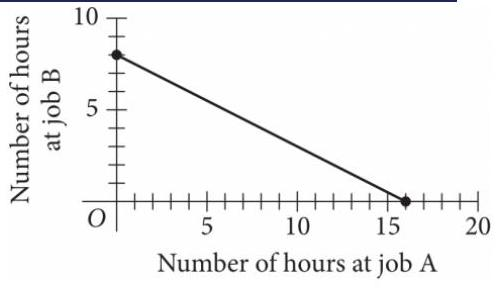
\includegraphics[max width=\textwidth, center]{2025_06_15_8c4b9d94a674ec08620fg-58}

To earn money for college, Avery works two part-time jobs: A and B. She earns \$10 per hour working at job A and $\$ 20$ per hour working at job B. In one week, Avery earned a total of $s$ dollars for working at the two part-time jobs. The graph above represents all possible combinations of numbers of hours Avery could have worked at the two jobs to earn $s$ dollars. What is the value of $s$ ?\\
A. 128\\
B. 160\\
C. 200\\
D. 320

\section*{ID: 029c2dc2}
A teacher is creating an assignment worth 70 points. The assignment will consist of questions worth 1 point and questions worth 3 points. Which equation represents this situation, where $x$ represents the number of 1 -point questions and $y$ represents the number of 3 -point questions?\\
A. $4 x y=70$\\
B. $4(x+y)=70$\\
C. $3 x+y=70$\\
D. $x+3 y=70$

\section*{ID: 2e1a7f66}
Figure $A$ and figure $B$ are both regular polygons. The sum of the perimeter of figure $A$ and the perimeter of figure $B$ is 63 inches. The equation $3 x+6 y=63$ represents this situation, where $x$ is the number of sides of figure A and $y$ is the number of sides of figure $B$. Which statement is the best interpretation of 6 in this context?\\
A. Each side of figure $B$ has a length of 6 inches.\\
B. The number of sides of figure $B$ is 6 .\\
C. Each side of figure $A$ has a length of 6 inches.\\
D. The number of sides of figure A is 6 .

\section*{ID: c5479c1a}
A shipment consists of 5 -pound boxes and 10 -pound boxes with a total weight of 220 pounds. There are 13 10-pound boxes in the shipment. How many 5 -pound boxes are in the shipment?\\
A. 5\\
B. 10\\
C. 13\\
D. 18

\section*{ID: 637022d2}
$$
2.5 b+5 r=80
$$

The given equation describes the relationship between the number of birds, $b$, and the number of reptiles, $r$, that can be cared for at a pet care business on a given day. If the business cares for 16 reptiles on a given day, how many birds can it care for on this day?\\
A. 0\\
B. 5\\
C. 40\\
D. 80

$$
y=70 x+8
$$

Which table gives three values of $x$ and their corresponding values of $y$ for the given equation?\\
A.

\begin{center}
\begin{tabular}{|c|c|}
\hline
$x$ & $y$ \\
\hline
0 & 8 \\
\hline
2 & 148 \\
\hline
4 & 288 \\
\hline
\end{tabular}
\end{center}

B.

\begin{center}
\begin{tabular}{|c|c|}
\hline
$x$ & $y$ \\
\hline
0 & 70 \\
\hline
2 & 78 \\
\hline
4 & 86 \\
\hline
\end{tabular}
\end{center}

c.

\begin{center}
\begin{tabular}{|c|c|}
\hline
$x$ & $y$ \\
\hline
0 & 70 \\
\hline
2 & 140 \\
\hline
4 & 280 \\
\hline
\end{tabular}
\end{center}

D.

\begin{center}
\begin{tabular}{|c|c|}
\hline
$x$ & $y$ \\
\hline
0 & 8 \\
\hline
2 & 132 \\
\hline
4 & 272 \\
\hline
\end{tabular}
\end{center}

The line with the equation $\frac{4}{5} x+\frac{1}{3} y=1$ is graphed in the $x y$-plane. What is the $x$-coordinate of the $x$-intercept of the line?\\
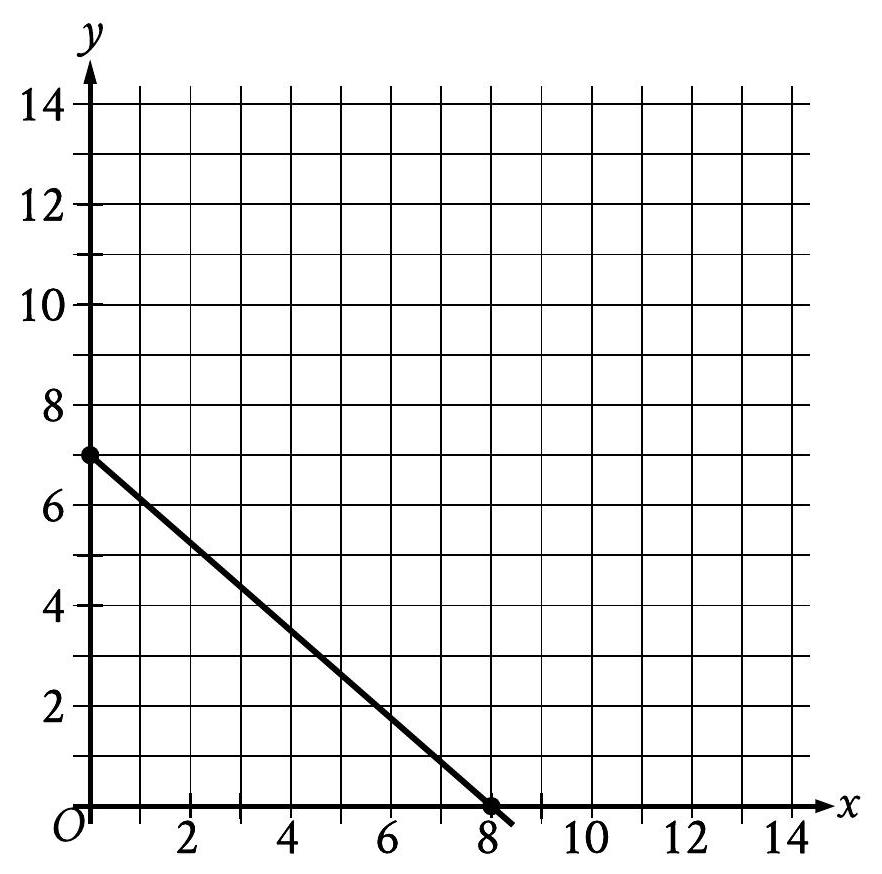
\includegraphics[max width=\textwidth, center]{2025_06_15_8c4b9d94a674ec08620fg-65}

The point with coordinates $(d, 4)$ lies on the line shown. What is the value of $d$ ?\\
A. $\frac{7}{2}$\\
B. $\frac{26}{7}$\\
C. $\frac{24}{7}$\\
D. $\frac{27}{8}$

\section*{ID: b9839f9e}
$F=2.50 x+7.00 y$

In the equation above, $F$ represents the total amount of money, in dollars, a food truck charges for $x$ drinks and $y$ salads. The price, in dollars, of each drink is the same, and the price, in dollars, of each salad is the same. Which of the following is the best interpretation for the number 7.00 in this context?\\
A. The price, in dollars, of one drink\\
B. The price, in dollars, of one salad\\
C. The number of drinks bought during the day\\
D. The number of salads bought during the day

\section*{ID: a7a14e87}
In the $x y$-plane, line $k$ is defined by $x+y=0$. Line $j$ is perpendicular to line $k$, and the $y$-intercept of line $j$ is $(0,3)$. Which of the following is an equation of line $j$ ?\\
A. $x+y=3$\\
B. $x+y=-3$\\
C. $x-y=3$\\
D. $x-y=-3$

\section*{ID: 6f6dfe3e}
\begin{center}
\begin{tabular}{|c|c|}
\hline
$x$ & $y$ \\
\hline
-6 & $n+184$ \\
\hline
-3 & $n+92$ \\
\hline
0 & $n$ \\
\hline
\end{tabular}
\end{center}

The table shows three values of $x$ and their corresponding values of $y$, where $n$ is a constant, for the linear relationship between $x$ and $y$. What is the slope of the line that represents this relationship in the $x y$-plane?\\
A. $-\frac{92}{3}$\\
B. $-\frac{3}{92}$\\
C. $\frac{n+92}{-3}$\\
D. $\frac{2 n-92}{3}$

\section*{ID: 038d87d7}
A neighborhood consists of a 2 -hectare park and a 35 -hectare residential area. The total number of trees in the neighborhood is 3,934 . The equation $2 x+35 y=3,934$ represents this situation. Which of the following is the best interpretation of $x$ in this context?\\
A. The average number of trees per hectare in the park\\
B. The average number of trees per hectare in the residential area\\
C. The total number of trees in the park\\
D. The total number of trees in the residential area

\section*{ID: 174885f8}
Jay walks at a speed of 3 miles per hour and runs at a speed of 5 miles per hour. He walks for $w$ hours and runs for $r$ hours for a combined total of 14 miles. Which equation represents this situation?\\
A. $3 w+5 r=14$\\
B. $\frac{1}{3} w+\frac{1}{5} r=14$\\
C. $\frac{1}{3} w+\frac{1}{5} r=112$\\
D. $3 w+5 r=112$

How many liters of a $25 \%$ saline solution must be added to 3 liters of a $10 \%$ saline solution to obtain a $15 \%$ saline solution?

What is the slope of the graph of $y=\frac{1}{4}(27 x+15)+7 x$ in the $x y$-plane?

\section*{ID: fb43b85f}
A line passes through the points $(4,6)$ and $(15,24)$ in the $x y$-plane. What is the slope of the line?\\
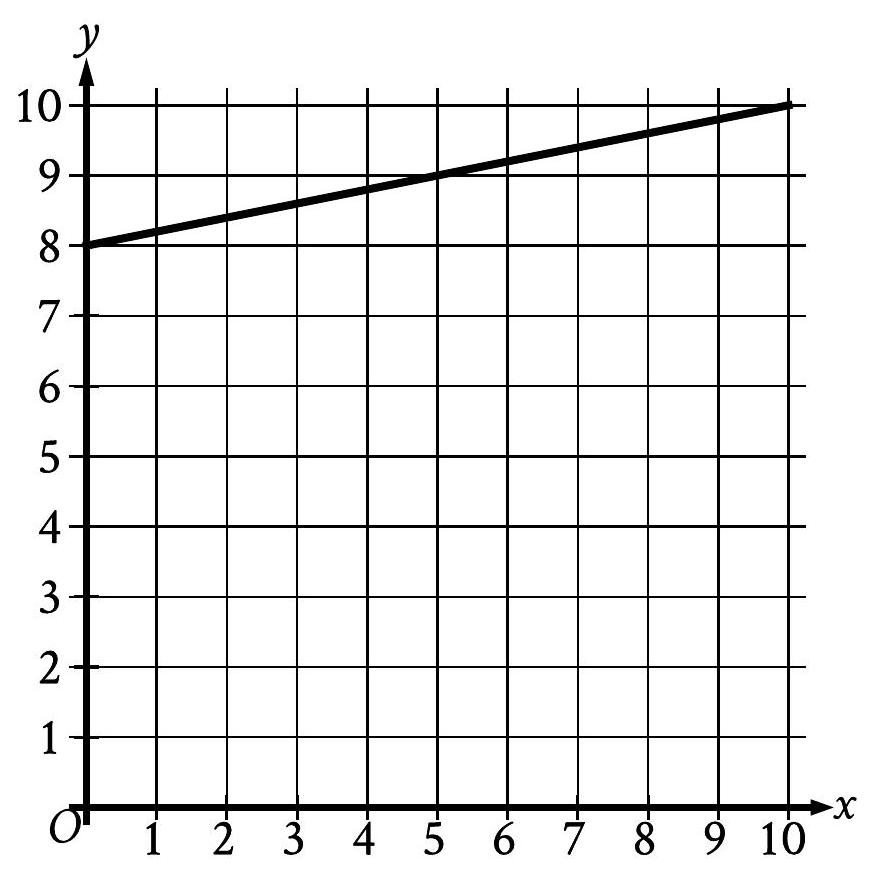
\includegraphics[max width=\textwidth, center]{2025_06_15_8c4b9d94a674ec08620fg-74}

What is the $y$-intercept of the line graphed?\\
A. $(0,-8)$\\
B. $\left(0,-\frac{1}{8}\right)$\\
C. $(0,0)$\\
D. $(0,8)$

The equation $46=2 a+2 b$ gives the relationship between the side lengths $a$ and $b$ of a certain parallelogram. If $a=9$, what is the value of $b$ ?

\section*{ID: 768b2425}
Last week, an interior designer earned a total of $\$ 1,258$ from consulting for $x$ hours and drawing up plans for $y$ hours. The equation $68 x+85 y=1,258$ represents this situation. Which of the following is the best interpretation of 68 in this context?\\
A. The interior designer earned $\$ 68$ per hour consulting last week.\\
B. The interior designer worked 68 hours drawing up plans last week.\\
C. The interior designer earned $\$ 68$ per hour drawing up plans last week.\\
D. The interior designer worked 68 hours consulting last week.

The $y$-intercept of the graph of $y=-6 x-32$ in the $x y$-plane is $(0, y)$. What is the value of $y ?$\\
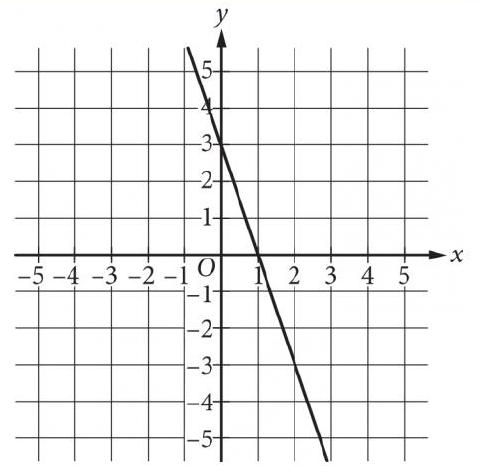
\includegraphics[max width=\textwidth, center]{2025_06_15_8c4b9d94a674ec08620fg-78}

What is the equation of the line shown in the $x y$-plane above?\\
A. $y=3 x-3$\\
B. $y=-3 x+3$\\
c. $y=\frac{1}{3} x-3$\\
D. $y=-\frac{1}{3} x+3$

\section*{ID: 535fa6e6}
Davio bought some potatoes and celery. The potatoes cost $\$ 0.69$ per pound, and the celery cost $\$ 0.99$ per pound. If Davio spent $\$ 5.34$ in total and bought twice as many pounds of celery as pounds of potatoes, how many pounds of celery did Davio buy?\\
A. 2\\
B. 2.5\\
C. 2.67\\
D. 4


